

\tikzset{every picture/.style={line width=0.75pt}} %set default line width to 0.75pt        

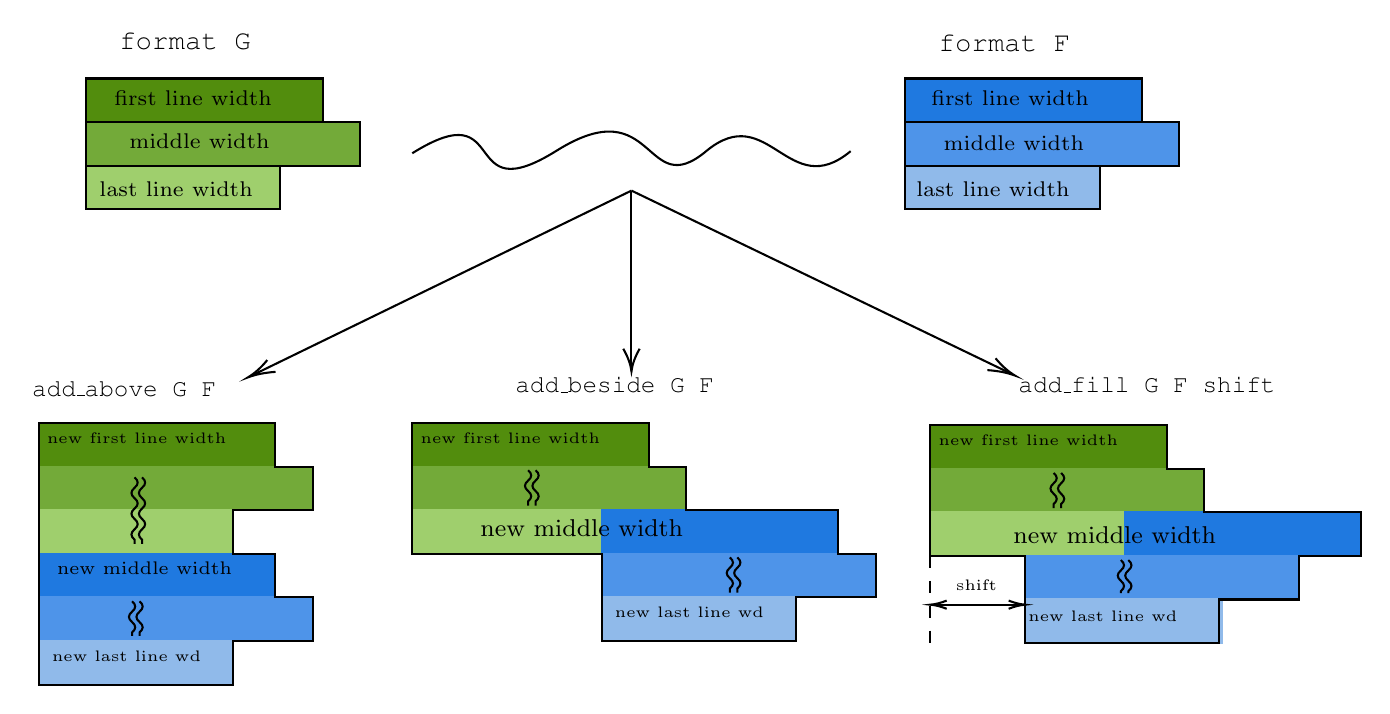
\begin{tikzpicture}[x=0.75pt,y=0.75pt,yscale=-1,xscale=1.2]
%uncomment if require: \path (0,446); %set diagram left start at 0, and has height of 446

%Curve Lines [id:da7282724148856031] 
\draw    (183,102) .. controls (223,72) and (201,130.73) .. (241,100.73) .. controls (281,70.73) and (276,126) .. (301,101) .. controls (326,76) and (334,126) .. (359,101) ;
%Straight Lines [id:da732226138129258] 
\draw    (271,120) -- (423.27,208.11) ;
\draw [shift={(425,209.12)}, rotate = 210.06] [color={rgb, 255:red, 0; green, 0; blue, 0 }  ][line width=0.75]    (10.93,-3.29) .. controls (6.95,-1.4) and (3.31,-0.3) .. (0,0) .. controls (3.31,0.3) and (6.95,1.4) .. (10.93,3.29)   ;
%Straight Lines [id:da2673745236113916] 
\draw    (271,120) -- (271,205.12) ;
\draw [shift={(271,207.12)}, rotate = 270] [color={rgb, 255:red, 0; green, 0; blue, 0 }  ][line width=0.75]    (10.93,-3.29) .. controls (6.95,-1.4) and (3.31,-0.3) .. (0,0) .. controls (3.31,0.3) and (6.95,1.4) .. (10.93,3.29)   ;
%Straight Lines [id:da5590791800548975] 
\draw    (271,120) -- (118.73,208.99) ;
\draw [shift={(117,210)}, rotate = 329.7] [color={rgb, 255:red, 0; green, 0; blue, 0 }  ][line width=0.75]    (10.93,-3.29) .. controls (6.95,-1.4) and (3.31,-0.3) .. (0,0) .. controls (3.31,0.3) and (6.95,1.4) .. (10.93,3.29)   ;
%Shape: Rectangle [id:dp808837789421493] 
\draw  [fill={rgb, 255:red, 82; green, 141; blue, 13 }  ,fill opacity=1 ] (52,66) -- (147,66) -- (147,87) -- (52,87) -- cycle ;
%Shape: Rectangle [id:dp9793592211997744] 
\draw  [fill={rgb, 255:red, 115; green, 170; blue, 57 }  ,fill opacity=1 ] (52,87) -- (162,87) -- (162,108) -- (52,108) -- cycle ;
%Shape: Rectangle [id:dp932877347953496] 
\draw  [fill={rgb, 255:red, 159; green, 207; blue, 109 }  ,fill opacity=1 ] (52,108) -- (130,108) -- (130,129) -- (52,129) -- cycle ;
%Shape: Rectangle [id:dp7757811105837442] 
\draw  [fill={rgb, 255:red, 31; green, 121; blue, 224 }  ,fill opacity=1 ] (381,66) -- (476,66) -- (476,87) -- (381,87) -- cycle ;
%Shape: Rectangle [id:dp9348863965428301] 
\draw  [fill={rgb, 255:red, 78; green, 148; blue, 233 }  ,fill opacity=1 ] (381,87) -- (491,87) -- (491,108) -- (381,108) -- cycle ;
%Shape: Rectangle [id:dp5258984646265605] 
\draw  [fill={rgb, 255:red, 144; green, 186; blue, 234 }  ,fill opacity=1 ] (381,108) -- (459,108) -- (459,129) -- (381,129) -- cycle ;
%Shape: Rectangle [id:dp001902336021333717] 
\draw  [color={rgb, 255:red, 82; green, 141; blue, 13 }  ,draw opacity=1 ][fill={rgb, 255:red, 82; green, 141; blue, 13 }  ,fill opacity=1 ] (33,232) -- (128,232) -- (128,253) -- (33,253) -- cycle ;
%Shape: Rectangle [id:dp4189646464121347] 
\draw  [color={rgb, 255:red, 115; green, 170; blue, 57 }  ,draw opacity=1 ][fill={rgb, 255:red, 115; green, 170; blue, 57 }  ,fill opacity=1 ] (33,253) -- (143,253) -- (143,274) -- (33,274) -- cycle ;
%Shape: Rectangle [id:dp6182085830852484] 
\draw  [color={rgb, 255:red, 159; green, 207; blue, 109 }  ,draw opacity=1 ][fill={rgb, 255:red, 159; green, 207; blue, 109 }  ,fill opacity=1 ] (33,274) -- (111,274) -- (111,295) -- (33,295) -- cycle ;
%Shape: Rectangle [id:dp279035114500889] 
\draw  [color={rgb, 255:red, 31; green, 121; blue, 224 }  ,draw opacity=1 ][fill={rgb, 255:red, 31; green, 121; blue, 224 }  ,fill opacity=1 ] (33,295) -- (128,295) -- (128,316) -- (33,316) -- cycle ;
%Shape: Rectangle [id:dp7094574853653807] 
\draw  [color={rgb, 255:red, 78; green, 148; blue, 233 }  ,draw opacity=1 ][fill={rgb, 255:red, 78; green, 148; blue, 233 }  ,fill opacity=1 ] (33,316) -- (143,316) -- (143,337) -- (33,337) -- cycle ;
%Shape: Rectangle [id:dp6311197532441868] 
\draw  [color={rgb, 255:red, 144; green, 186; blue, 234 }  ,draw opacity=1 ][fill={rgb, 255:red, 144; green, 186; blue, 234 }  ,fill opacity=1 ] (33,337) -- (111,337) -- (111,358) -- (33,358) -- cycle ;
%Shape: Rectangle [id:dp005304650175637082] 
\draw  [color={rgb, 255:red, 82; green, 141; blue, 13 }  ,draw opacity=1 ][fill={rgb, 255:red, 82; green, 141; blue, 13 }  ,fill opacity=1 ] (183,232) -- (278,232) -- (278,253) -- (183,253) -- cycle ;
%Shape: Rectangle [id:dp1795210702408092] 
\draw  [color={rgb, 255:red, 115; green, 170; blue, 57 }  ,draw opacity=1 ][fill={rgb, 255:red, 115; green, 170; blue, 57 }  ,fill opacity=1 ] (183,253) -- (293,253) -- (293,274) -- (183,274) -- cycle ;
%Shape: Rectangle [id:dp281817417555301] 
\draw  [color={rgb, 255:red, 159; green, 207; blue, 109 }  ,draw opacity=1 ][fill={rgb, 255:red, 159; green, 207; blue, 109 }  ,fill opacity=1 ] (183,274) -- (261,274) -- (261,295) -- (183,295) -- cycle ;
%Shape: Rectangle [id:dp2764643146730045] 
\draw  [color={rgb, 255:red, 31; green, 121; blue, 224 }  ,draw opacity=1 ][fill={rgb, 255:red, 31; green, 121; blue, 224 }  ,fill opacity=1 ] (259,274) -- (354,274) -- (354,295) -- (259,295) -- cycle ;
%Shape: Rectangle [id:dp14893535880956488] 
\draw  [color={rgb, 255:red, 78; green, 148; blue, 233 }  ,draw opacity=1 ][fill={rgb, 255:red, 78; green, 148; blue, 233 }  ,fill opacity=1 ] (259,295) -- (369,295) -- (369,316) -- (259,316) -- cycle ;
%Shape: Rectangle [id:dp1374086019688595] 
\draw  [color={rgb, 255:red, 144; green, 186; blue, 234 }  ,draw opacity=1 ][fill={rgb, 255:red, 144; green, 186; blue, 234 }  ,fill opacity=1 ] (259,316) -- (337,316) -- (337,337) -- (259,337) -- cycle ;
%Shape: Rectangle [id:dp23030297917489972] 
\draw  [color={rgb, 255:red, 82; green, 141; blue, 13 }  ,draw opacity=1 ][fill={rgb, 255:red, 82; green, 141; blue, 13 }  ,fill opacity=1 ] (391,233) -- (486,233) -- (486,254) -- (391,254) -- cycle ;
%Shape: Rectangle [id:dp8602353837487641] 
\draw  [color={rgb, 255:red, 115; green, 170; blue, 57 }  ,draw opacity=1 ][fill={rgb, 255:red, 115; green, 170; blue, 57 }  ,fill opacity=1 ] (391,254) -- (501,254) -- (501,275) -- (391,275) -- cycle ;
%Shape: Rectangle [id:dp17203495759689613] 
\draw  [color={rgb, 255:red, 159; green, 207; blue, 109 }  ,draw opacity=1 ][fill={rgb, 255:red, 159; green, 207; blue, 109 }  ,fill opacity=1 ] (391,275) -- (469,275) -- (469,296) -- (391,296) -- cycle ;
%Shape: Rectangle [id:dp7376664524660743] 
\draw  [color={rgb, 255:red, 31; green, 121; blue, 224 }  ,draw opacity=1 ][fill={rgb, 255:red, 31; green, 121; blue, 224 }  ,fill opacity=1 ] (469,275) -- (564,275) -- (564,296) -- (469,296) -- cycle ;
%Shape: Rectangle [id:dp7450826439827496] 
\draw  [color={rgb, 255:red, 78; green, 148; blue, 233 }  ,draw opacity=1 ][fill={rgb, 255:red, 78; green, 148; blue, 233 }  ,fill opacity=1 ] (429,296) -- (539,296) -- (539,317) -- (429,317) -- cycle ;
%Shape: Rectangle [id:dp8041860035178171] 
\draw  [color={rgb, 255:red, 144; green, 186; blue, 234 }  ,draw opacity=1 ][fill={rgb, 255:red, 144; green, 186; blue, 234 }  ,fill opacity=1 ] (430,317) -- (508,317) -- (508,338) -- (430,338) -- cycle ;
%Shape: Polygon [id:ds9630730212561414] 
\draw   (128,253) -- (143,253) -- (143,274) -- (111,274) -- (111,295) -- (128,295) -- (128,316) -- (143,316) -- (143,337) -- (111,337) -- (111,358) -- (33,358) -- (33,232) -- (128,232) -- cycle ;
%Shape: Polygon [id:ds6875341607963043] 
\draw   (183,232) -- (278,232) -- (278,253) -- (293,253) -- (293,274) -- (354,274) -- (354,295) -- (369,295) -- (369,316) -- (337,316) -- (337,337) -- (259,337) -- (259,295) -- (183,295) -- cycle ;
%Shape: Polygon [id:ds7737589105011929] 
\draw   (391,233) -- (486,233) -- (486,254) -- (501,254) -- (501,275) -- (564,275) -- (564,296) -- (539,296) -- (539,317) -- (507,317) -- (507,338) -- (429,338) -- (429,296) -- (391,296) -- cycle ;
%Straight Lines [id:da3118774411427221] 
\draw [line width=0.75]    (74.5,258.18) .. controls (76.17,259.85) and (76.17,261.51) .. (74.5,263.18) .. controls (72.83,264.85) and (72.83,266.51) .. (74.5,268.18) .. controls (76.17,269.85) and (76.17,271.51) .. (74.5,273.18) .. controls (72.83,274.85) and (72.83,276.51) .. (74.5,278.18) .. controls (76.17,279.85) and (76.17,281.51) .. (74.5,283.18) .. controls (72.83,284.85) and (72.83,286.51) .. (74.5,288.18) -- (74.5,290.18) -- (74.5,290.18)(71.5,258.18) .. controls (73.17,259.85) and (73.17,261.51) .. (71.5,263.18) .. controls (69.83,264.85) and (69.83,266.51) .. (71.5,268.18) .. controls (73.17,269.85) and (73.17,271.51) .. (71.5,273.18) .. controls (69.83,274.85) and (69.83,276.51) .. (71.5,278.18) .. controls (73.17,279.85) and (73.17,281.51) .. (71.5,283.18) .. controls (69.83,284.85) and (69.83,286.51) .. (71.5,288.18) -- (71.5,290.18) -- (71.5,290.18) ;
%Straight Lines [id:da2560676519649512] 
\draw [line width=0.75]    (73.5,317.87) .. controls (75.17,319.54) and (75.17,321.2) .. (73.5,322.87) .. controls (71.83,324.54) and (71.83,326.2) .. (73.5,327.87) .. controls (75.17,329.54) and (75.17,331.2) .. (73.5,332.87) -- (73.5,334.5) -- (73.5,334.5)(70.5,317.87) .. controls (72.17,319.54) and (72.17,321.2) .. (70.5,322.87) .. controls (68.83,324.54) and (68.83,326.2) .. (70.5,327.87) .. controls (72.17,329.54) and (72.17,331.2) .. (70.5,332.87) -- (70.5,334.5) -- (70.5,334.5) ;
%Straight Lines [id:da03198072222338155] 
\draw [line width=0.75]    (232.5,254.73) .. controls (234.17,256.4) and (234.17,258.06) .. (232.5,259.73) .. controls (230.83,261.4) and (230.83,263.06) .. (232.5,264.73) .. controls (234.17,266.4) and (234.17,268.06) .. (232.5,269.73) -- (232.5,271.73) -- (232.5,271.73)(229.5,254.73) .. controls (231.17,256.4) and (231.17,258.06) .. (229.5,259.73) .. controls (227.83,261.4) and (227.83,263.06) .. (229.5,264.73) .. controls (231.17,266.4) and (231.17,268.06) .. (229.5,269.73) -- (229.5,271.73) -- (229.5,271.73) ;
%Straight Lines [id:da19304958682708773] 
\draw [line width=0.75]    (313.5,296.73) .. controls (315.17,298.4) and (315.17,300.06) .. (313.5,301.73) .. controls (311.83,303.4) and (311.83,305.06) .. (313.5,306.73) .. controls (315.17,308.4) and (315.17,310.06) .. (313.5,311.73) -- (313.5,313.73) -- (313.5,313.73)(310.5,296.73) .. controls (312.17,298.4) and (312.17,300.06) .. (310.5,301.73) .. controls (308.83,303.4) and (308.83,305.06) .. (310.5,306.73) .. controls (312.17,308.4) and (312.17,310.06) .. (310.5,311.73) -- (310.5,313.73) -- (310.5,313.73) ;
%Straight Lines [id:da5516188067826676] 
\draw [line width=0.75]    (443.5,256.03) .. controls (445.17,257.7) and (445.17,259.36) .. (443.5,261.03) .. controls (441.83,262.7) and (441.83,264.36) .. (443.5,266.03) .. controls (445.17,267.7) and (445.17,269.36) .. (443.5,271.03) -- (443.5,273.03) -- (443.5,273.03)(440.5,256.03) .. controls (442.17,257.7) and (442.17,259.36) .. (440.5,261.03) .. controls (438.83,262.7) and (438.83,264.36) .. (440.5,266.03) .. controls (442.17,267.7) and (442.17,269.36) .. (440.5,271.03) -- (440.5,273.03) -- (440.5,273.03) ;
%Straight Lines [id:da6746831310479344] 
\draw [line width=0.75]    (470.5,298) .. controls (472.17,299.67) and (472.17,301.33) .. (470.5,303) .. controls (468.83,304.67) and (468.83,306.33) .. (470.5,308) .. controls (472.17,309.67) and (472.17,311.33) .. (470.5,313) -- (470.5,313.97) -- (470.5,313.97)(467.5,298) .. controls (469.17,299.67) and (469.17,301.33) .. (467.5,303) .. controls (465.83,304.67) and (465.83,306.33) .. (467.5,308) .. controls (469.17,309.67) and (469.17,311.33) .. (467.5,313) -- (467.5,313.97) -- (467.5,313.97) ;
%Straight Lines [id:da6479439546727871] 
\draw  [dash pattern={on 4.5pt off 4.5pt}]  (391,296) -- (391,339) ;
%Straight Lines [id:da82336201819135] 
\draw    (393,319.5) -- (427,319.5) ;
\draw [shift={(429,319.5)}, rotate = 180] [color={rgb, 255:red, 0; green, 0; blue, 0 }  ][line width=0.75]    (6.56,-1.97) .. controls (4.17,-0.84) and (1.99,-0.18) .. (0,0) .. controls (1.99,0.18) and (4.17,0.84) .. (6.56,1.97)   ;
\draw [shift={(391,319.5)}, rotate = 0] [color={rgb, 255:red, 0; green, 0; blue, 0 }  ][line width=0.75]    (6.56,-1.97) .. controls (4.17,-0.84) and (1.99,-0.18) .. (0,0) .. controls (1.99,0.18) and (4.17,0.84) .. (6.56,1.97)   ;

% Text Node
\draw (64,42) node [anchor=north west][inner sep=0.75pt]  [color={rgb, 255:red, 0; green, 0; blue, 0 }  ,opacity=1 ,xscale=1.1,yscale=1.1] [align=left] {{\fontfamily{pcr}\selectfont {\small format G}}};
% Text Node
\draw (29,210) node [anchor=north west][inner sep=0.75pt]  [xscale=1.1,yscale=1.1] [align=left] {{\footnotesize {\fontfamily{pcr}\selectfont add\_above G F}}};
% Text Node
\draw (223,208) node [anchor=north west][inner sep=0.75pt]  [xscale=1.1,yscale=1.1] [align=left] {{\footnotesize {\fontfamily{pcr}\selectfont add\_beside G F}}};
% Text Node
\draw (425,208) node [anchor=north west][inner sep=0.75pt]  [xscale=1.1,yscale=1.1] [align=left] {{\footnotesize {\fontfamily{pcr}\selectfont add\_fill G F shift}}};
% Text Node
\draw (62,70) node [anchor=north west][inner sep=0.75pt]  [xscale=1.1,yscale=1.1] [align=left] {{\fontfamily{helvet}\selectfont {\scriptsize first line width}}};
% Text Node
\draw (68,91) node [anchor=north west][inner sep=0.75pt]  [xscale=1.1,yscale=1.1] [align=left] {{\scriptsize middle width}};
% Text Node
\draw (56,114) node [anchor=north west][inner sep=0.75pt]  [xscale=1.1,yscale=1.1] [align=left] {{\scriptsize last line width}};
% Text Node
\draw (393,43) node [anchor=north west][inner sep=0.75pt]  [color={rgb, 255:red, 0; green, 0; blue, 0 }  ,opacity=1 ,xscale=1.1,yscale=1.1] [align=left] {{\fontfamily{pcr}\selectfont {\small format F}}};
% Text Node
\draw (35,235) node [anchor=north west][inner sep=0.75pt]  [color={rgb, 255:red, 0; green, 0; blue, 0 }  ,opacity=1 ,xscale=1.1,yscale=1.1] [align=left] {{\fontfamily{helvet}\selectfont {\fontsize{0.53em}{0.64em}\selectfont new first line width}}};
% Text Node
\draw (37,340) node [anchor=north west][inner sep=0.75pt]  [color={rgb, 255:red, 0; green, 0; blue, 0 }  ,opacity=1 ,xscale=1.1,yscale=1.1] [align=left] {{\fontfamily{helvet}\selectfont {\fontsize{0.53em}{0.64em}\selectfont new last line wd}}};
% Text Node
\draw (39,297) node [anchor=north west][inner sep=0.75pt]  [color={rgb, 255:red, 0; green, 0; blue, 0 }  ,opacity=1 ,rotate=-0.02,xscale=1.1,yscale=1.1] [align=left] {{\fontsize{0.6em}{0.72em}\selectfont new middle width}};
% Text Node
\draw (390,70) node [anchor=north west][inner sep=0.75pt]  [xscale=1.1,yscale=1.1] [align=left] {{\fontfamily{helvet}\selectfont {\scriptsize first line width}}};
% Text Node
\draw (395,92) node [anchor=north west][inner sep=0.75pt]  [xscale=1.1,yscale=1.1] [align=left] {{\scriptsize middle width}};
% Text Node
\draw (384,114) node [anchor=north west][inner sep=0.75pt]  [xscale=1.1,yscale=1.1] [align=left] {{\scriptsize last line width}};
% Text Node
\draw (185,235) node [anchor=north west][inner sep=0.75pt]  [color={rgb, 255:red, 0; green, 0; blue, 0 }  ,opacity=1 ,xscale=1.1,yscale=1.1] [align=left] {{\fontfamily{helvet}\selectfont {\fontsize{0.53em}{0.64em}\selectfont new first line width}}};
% Text Node
\draw (209,277) node [anchor=north west][inner sep=0.75pt]  [color={rgb, 255:red, 0; green, 0; blue, 0 }  ,opacity=1 ,rotate=-0.02,xscale=1.1,yscale=1.1] [align=left] {{\footnotesize new middle width}};
% Text Node
\draw (263,319) node [anchor=north west][inner sep=0.75pt]  [color={rgb, 255:red, 0; green, 0; blue, 0 }  ,opacity=1 ,xscale=1.1,yscale=1.1] [align=left] {{\fontfamily{helvet}\selectfont {\fontsize{0.53em}{0.64em}\selectfont new last line wd}}};
% Text Node
\draw (393,236) node [anchor=north west][inner sep=0.75pt]  [color={rgb, 255:red, 0; green, 0; blue, 0 }  ,opacity=1 ,xscale=1.1,yscale=1.1] [align=left] {{\fontfamily{helvet}\selectfont {\fontsize{0.53em}{0.64em}\selectfont new first line width}}};
% Text Node
\draw (423,280) node [anchor=north west][inner sep=0.75pt]  [color={rgb, 255:red, 0; green, 0; blue, 0 }  ,opacity=1 ,rotate=-0.02,xscale=1.1,yscale=1.1] [align=left] {{\footnotesize new middle width}};
% Text Node
\draw (429,321) node [anchor=north west][inner sep=0.75pt]  [color={rgb, 255:red, 0; green, 0; blue, 0 }  ,opacity=1 ,xscale=1.1,yscale=1.1] [align=left] {{\fontfamily{helvet}\selectfont {\fontsize{0.53em}{0.64em}\selectfont new last line wd}}};
% Text Node
\draw (400,306) node [anchor=north west][inner sep=0.75pt]  [xscale=1.1,yscale=1.1] [align=left] {{\tiny shift}};


\end{tikzpicture}
